%!TEX root = stokes_paper.tex

\section{Numerical examples}
In this section, we present contour plots for the stream function $\psi$ superimposed on a colorplor of the velocity magnitude. We use black contours for the first eddy and the subsequent ones are highlighted in yellow. The convergence plots indicate root-exponential convergence as expected. We also provide a close up of the eddies. We choose various popular sample problems found in the literature for testing the Lighting Stokes Solver. 

\subsection{Bounded, simply-connected domains}

\begin{figure}[H]
	\centering
	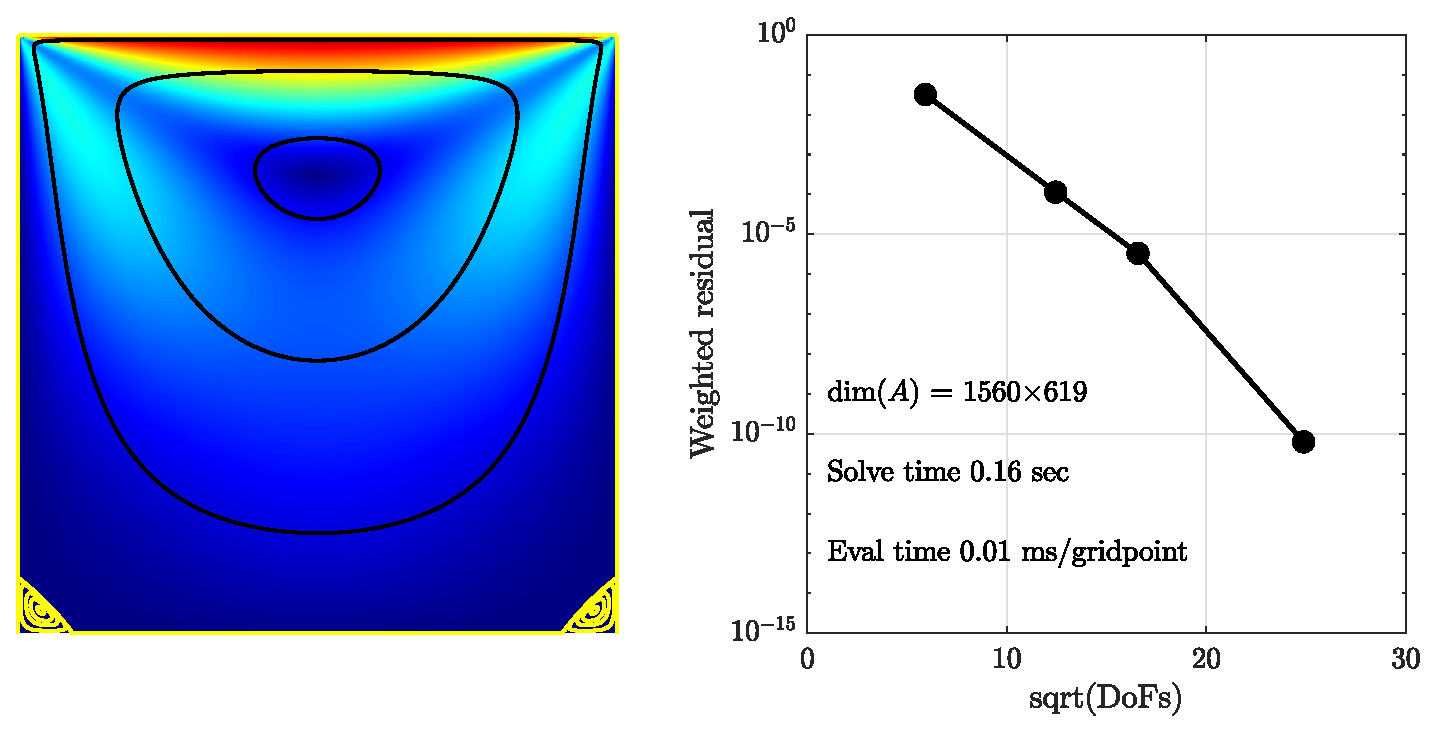
\includegraphics[width=\linewidth]{Figures/ldc}
	
	\vspace{2em}
	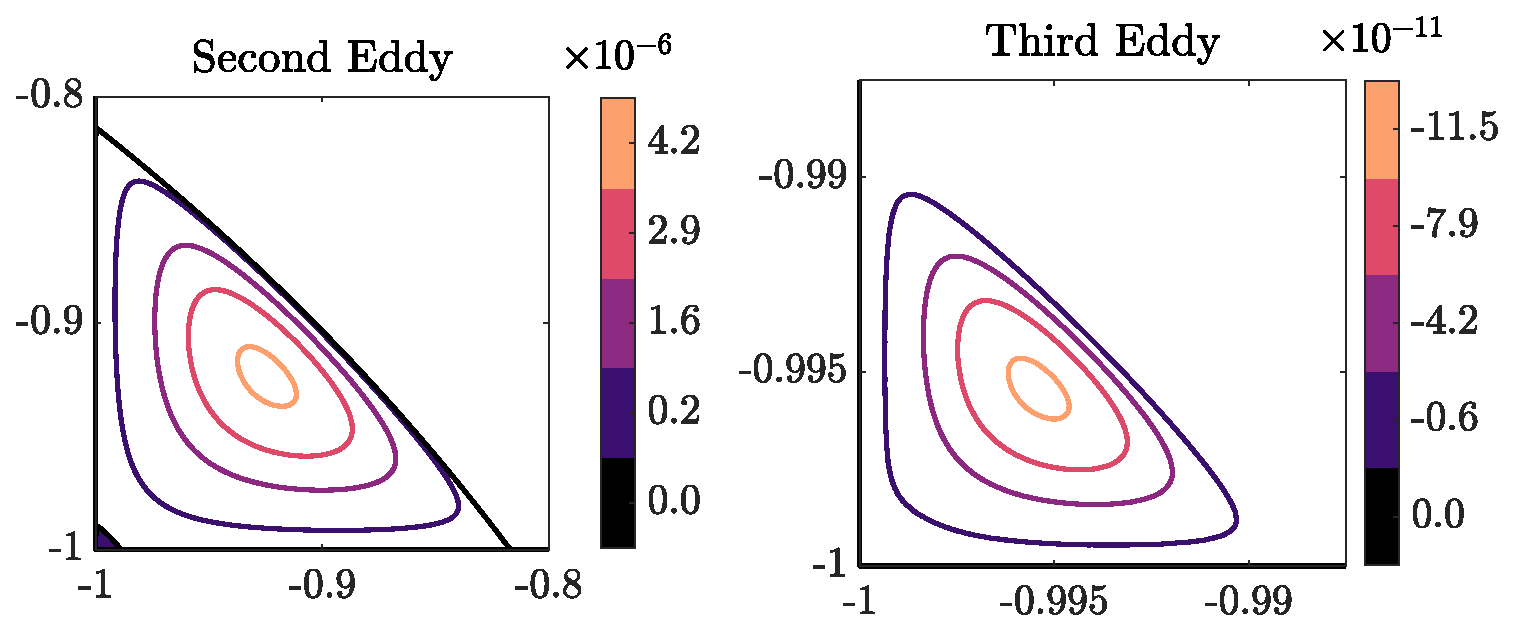
\includegraphics[width=\linewidth]{Figures/ldc_eddy}
	\label{fig:ldc}
	\caption{Stokes flow inside a square lid-driven cavity. In this example, a fluid is enclosed inside a cavity, whose lid moves from left to right with unit speed, and no-slip boundary conditions are imposed at the other 2 surfaces.}
\end{figure} 

\begin{figure}[H]
	\centering
	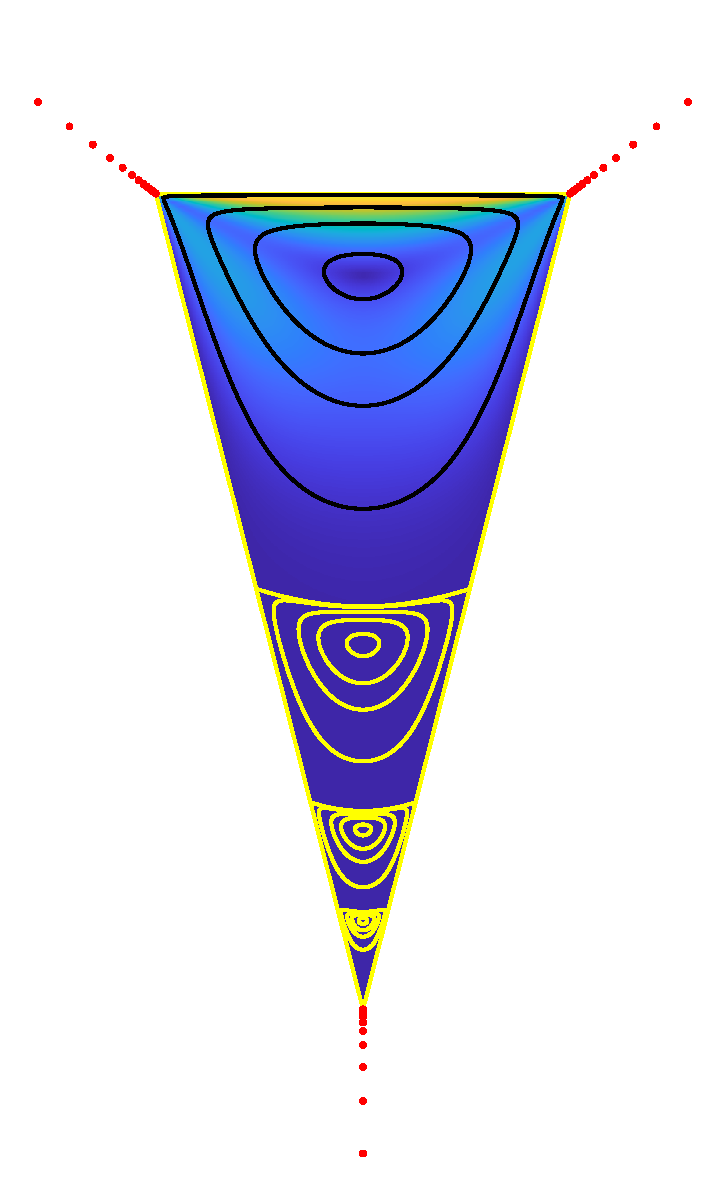
\includegraphics[width=\linewidth]{Figures/wedge}
	\label{fig:wedge}
	\caption{Stokes flow inside a wedge of total angle $28.5^\circ$. The top lid moves from left to right with unit speed and no-slip boundary conditions are imposed at the other 2 surfaces. For comparison, Ronquist, in \cite[Fig.~12]{Ronquist88}, solved the same problem with the spectral element method with $E=30$ and polynomial degree $N=8$, and no special treatment for the corners. which gives $\sqrt{\text{DoFs}}\approx 126$. The first two eddies have been observed experimentally by Taneda in \cite[Fig.~19]{Taneda79}, also included in \cite[Fig.~10]{VanDyke82}, for a very similar setup driven by a rotating cylinder with $\text{Re}=1.7\times10^{-1}$.}
\end{figure} 

\begin{figure}[H]
	\centering
	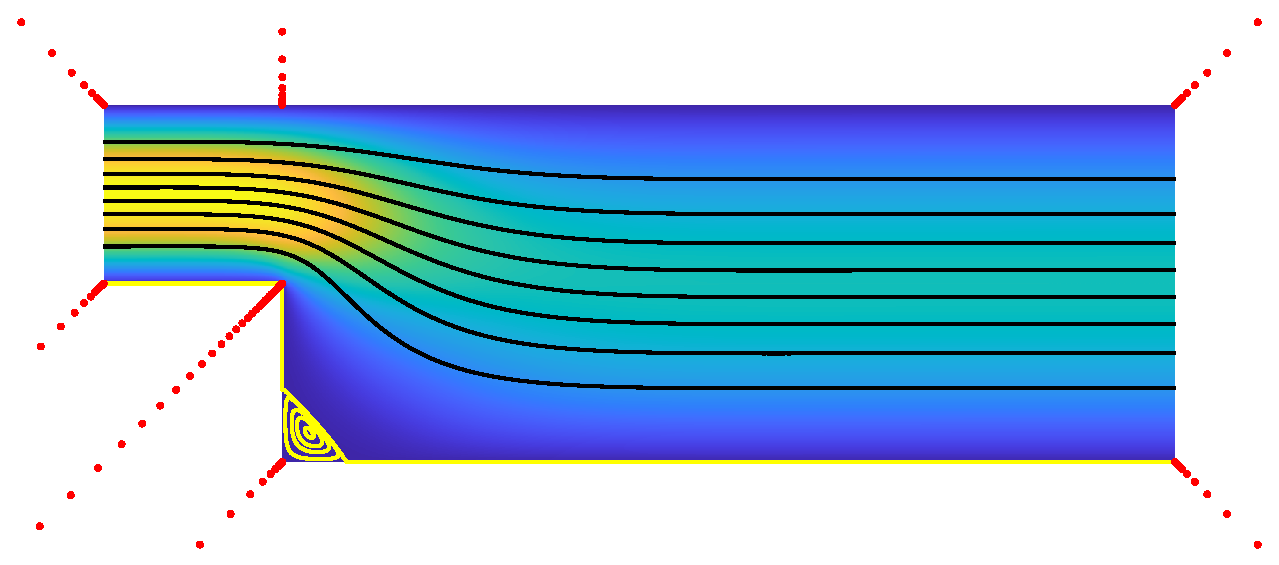
\includegraphics[width=\linewidth]{Figures/step}
	
	\vspace{2em}
	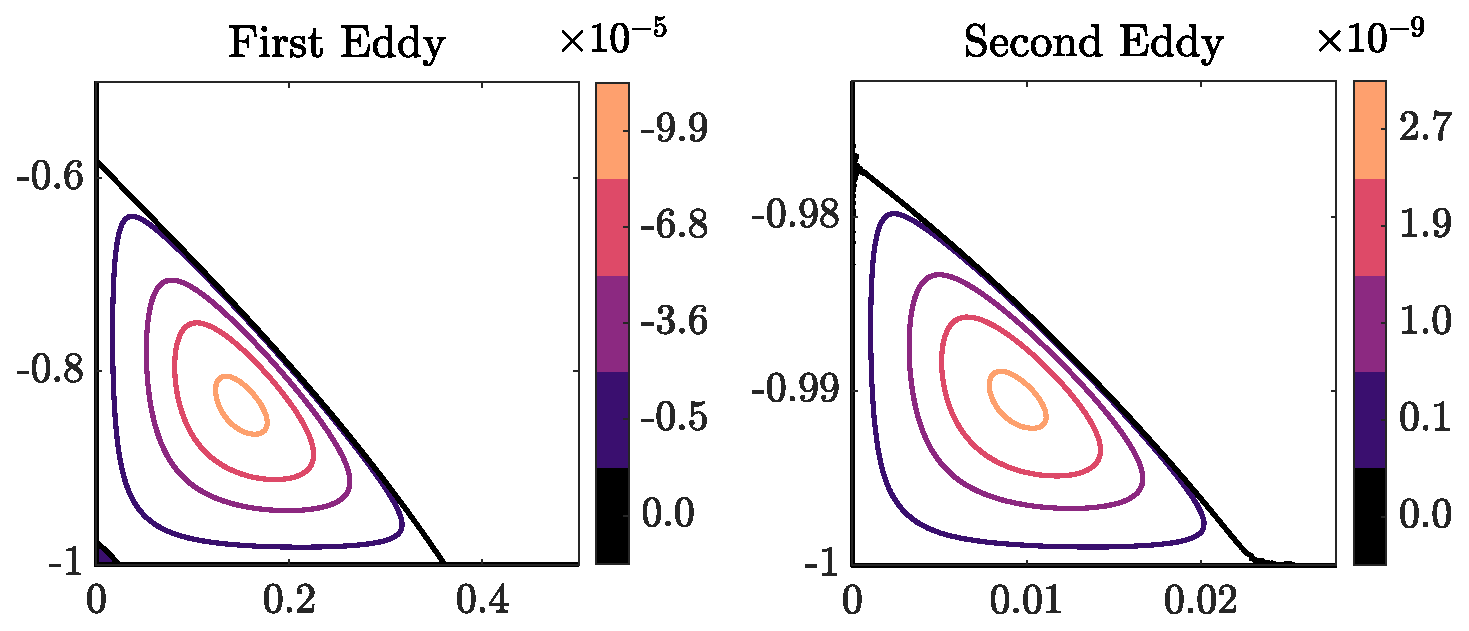
\includegraphics[width=\linewidth]{Figures/step_eddy}
	
	\vspace{2em}
	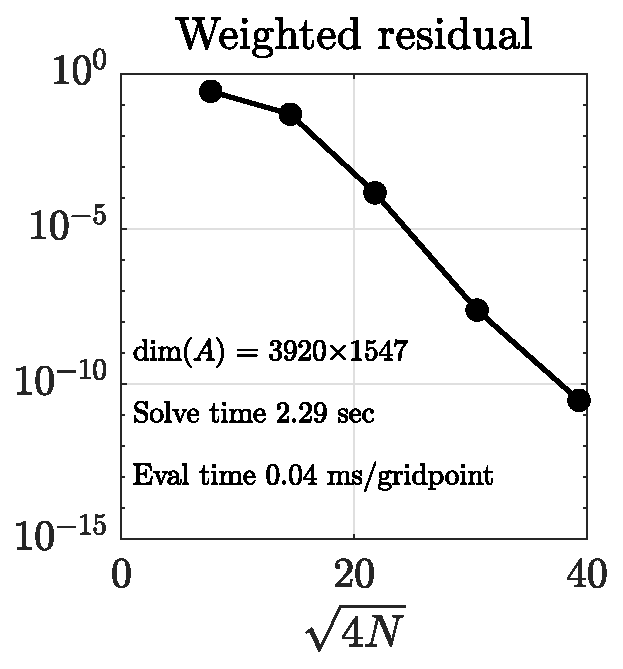
\includegraphics[width=0.5\linewidth]{Figures/step_conv}
	
	\label{fig:step}
	\caption{Stokes flow over a step. A parabolic profile is prescribed at the inflow and at the outflow, a no-slip condition is imposed on the rest of the walls. At the re-entrant corner the pressure and the derivatives of the velocity become unbounded.}
\end{figure} 

\subsection{Unbounded domains}

\subsection{Multiply connected domains}


The analytical solution for the flow past a cylinder of radius $R$ at a distance $d$ from an infinite wall was given by Wannier in \cite{Wannier50}
\begin{equation}
\psi = (A + Fy)\log \frac{x^2 + (s+y)^2}{x^2 + (s-y)^2} + B \frac{y(s+y)}{x^2 + (s+y)^2} + C \frac{y(s-y)}{x^2+(s-y)^2} + Dy + E\left(x^2+y^2+s^2\right).
\end{equation}
where $s^2=d^2-R^2$, and $A,B,C,D,E,F$ are constants to be determined.


